%%
%% This is file `sample-sigconf.tex',
%% generated with the docstrip utility.
%%
%% The original source files were:
%%
%% samples.dtx  (with options: `sigconf')
%% 
%% IMPORTANT NOTICE:
%% 
%% For the copyright see the source file.
%% 
%% Any modified versions of this file must be renamed
%% with new filenames distinct from sample-sigconf.tex.
%% 
%% For distribution of the original source see the terms
%% for copying and modification in the file samples.dtx.
%% 
%% This generated file may be distributed as long as the
%% original source files, as listed above, are part of the
%% same distribution. (The sources need not necessarily be
%% in the same archive or directory.)
%%
%% The first command in your LaTeX source must be the \documentclass command.
\documentclass[sigconf, nonacm, natbib, screen, balance=False]{acmart}

% Documentation for packages
% - ACM Article Template
%    https://www.acm.org/publications/proceedings-template
% - Pseudocode typesetting CLRS-style:
%    https://www.cs.dartmouth.edu/~thc/clrscode/clrscode3e.pdf
% - Python code typesetting
%    http://ctan.uib.no/macros/latex/contrib/listings/listings.pdf
% - AMS Math
%    http://ctan.uib.no/macros/latex/required/amsmath/amsldoc.pdf
% - Graphics
%    http://ctan.uib.no/macros/latex/required/graphics/grfguide.pdf

\usepackage{clrscode3e}  
\usepackage{listings}
\lstset{language=Python, basicstyle=\ttfamily}

% based on https://tex.stackexchange.com/questions/279240/float-for-lstlisting
\usepackage{float}
\floatstyle{ruled}
\newfloat{listing}{tbph}{lop}
\floatname{listing}{Listing}
\def\lstfloatautorefname{Listing} % needed for hyperref/auroref

\citestyle{acmauthoryear}

%% end of the preamble, start of the body of the document source.
\begin{document}

%%
%% The "title" command has an optional parameter,
%% allowing the author to define a "short title" to be used in page headers.
\title{Benchmarking Sorting Algorithms In Python}
\subtitle{INF221 Term Paper, NMBU, Autumn 2020}

\author{Jon-Mikkel Korsvik}
\email{jonkors@nmbu.no}
\affiliation{}  % separates Jane's and Joe's author block

\author{Yva Sandvik}
\email{ysandvik@nmbu.no}

%% The abstract is a short summary of the work to be presented in the
%% article.
\begin{abstract}
  In this paper, we analyse \dots 
\end{abstract}


%%
%% This command processes the author and affiliation and title
%% information and builds the first part of the formatted document.
\maketitle

\section{Introduction}\label{sec:intro}

Sorting algorithms are used to solve one of the key problems of computer science known as “The sorting problem”. This involves an input sequence of n numbers $(a_1, a_2, … , a_n)$, where the output is a permutation of the input sequence such that the numbers are ordered in an ascending order. The two main aspects to a sorting algorithm is its time complexity (speed) and its space complexity (memory usage). (Kilde: Lecture 6 ipynb, Plesser)

During this investigation we have assessed the performance of these sorting algorithms under certain assumptions regarding their time complexity. We explored their efficiency depending on the type of elements in a list that are to be sorted, as well as the length of the lists. 

In the following subsections we will provide theory, pseudocode as well as details surrounding the methods used when comparing the following sorting algorithms: 
\begin{itemize}
\item Quadratic algorithms
  \begin{itemize}
  \item insertion sort
  \item bubble sort
  \end{itemize}
\item Sub-quadratic algorithms
  \begin{itemize}
  \item mergesort
  \item quicksort
  \end{itemize}
\item Combined algorithm
  \begin{itemize}
  \item mergesort switching to insertion sort for small data
  \end{itemize}
\item Built-in sorting functions
  \begin{itemize}
  \item Python `sort()`
  \item NumPy `sort()`
  \end{itemize}
\item Possibly a few more if we have enough time
  \begin{itemize}
  \item Radix sort
  \item Heap sort
  \end{itemize}
\end{itemize}

\section{Theory}\label{sec:theory}

The first two algorithms we analyse are the quadratic sorting algorithms insertion sort and bubble sort. These two sorting algorithms are known as quadratic sorting algorithms because their Big O time complexity is $O(n^2)$.

Insertion sort is a simple comparison based sorting algorithm that iterates through a list one step at and starts by looking at the second value in an array and compares it to the one before, finding the correct position for the value in the sorted end of the input list (left side).

Bubble sort...

\subsection{Algorithm 1 - Insertion sort}\label{sec:algo1}

\begin{listing}
  % Pseudocode caption above the code.
  \caption{Insertion sort algorithm from \citet[Ch.~2.1]{CLRS_2009}.}
  \label{lst:insertion_algo}

  \begin{codebox}
    \Procname{$\proc{Insertion-Sort}(A)$}
    \li \For $j \gets 2$ \To $\attrib{A}{length}$
    \li \Do
    $\id{key} \gets A[j]$
    \li     $i \gets j-1$
    \li      \While $i>0$ and $A[i] > \id{key}$
    \li      \Do
    $A[i+1] \gets A[i]$
    \li         $i \gets i-1$
    \End    
    \li       $A[i+1]\gets \id{key}$
    \End
  \end{codebox}
\end{listing}

Pseudocode for the insertion sort is shown in
listing~\ref{lst:insertion_algo}. 
Best case runtime for this algorithm is:

\begin{equation}
  T(n) = \Theta(n) \;.  \label{eq:ins_sort_best}
\end{equation}

This is achieved when the input array is already sorted. Meaning the input value in each iteration is only compared to the rightmost value of the sorted list. 

Worst case runtime occurs if the input list is in reversed order. This gives a quadratic running time:

\begin{equation}
  T(n) = \Theta(n^2) \;.  \label{eq:ins_sort_best}
\end{equation}

The average runtime is also quadratic, making insertion sort a bad choice for sorting large lists, however it is one of the best and quickest alternatives when it comes to sorting smaller lists. 

We are going to compare insertion sort to several other comparison based sorting algorithms, such as bubble sort, quick sort and merge sort.

\subsection{Algorithm 2 - Bubble sort}\label{sec:algo2}

\begin{listing}
  % Pseudocode caption above the code.
  \caption{Bubble sort algorithm from \citet[Ch.~2.1]{CLRS_2009}.}
  \label{lst:bubble_algo}
 
  \begin{codebox}
    \Procname{$\proc{Bubble Sort}(A)$}
    \li $swapped = true$

  \end{codebox}
\end{listing}

Pseudocode for the bubble sort is shown in listing~\ref{lst:bubble_algo}. 

\subsection{Algorithm 3 - Merge sort}\label{sec:algo2}

\begin{listing}
  % Pseudocode caption above the code.
  \caption{Merge sort algorithm from \citet[Ch.~2.1]{CLRS_2009}.}
  \label{lst:merge_algo}

  \begin{codebox}
    \Procname{$\proc{Merge Sort}(A)$}

  \end{codebox}
\end{listing}

Pseudocode for the merge sort algorithm is shown in listing~\ref{lst:merge_algo}. 

\subsection{Algorithm 4 - Quick sort}\label{sec:algo2}

\begin{listing}
  % Pseudocode caption above the code.
  \caption{Quick sort algorithm from \citet[Ch.~2.1]{CLRS_2009}.}
  \label{lst:quick_algo}
  
  \begin{codebox}
    \Procname{$\proc{Quick Sort}(A)$}

  \end{codebox}
\end{listing}

Pseudocode for the quick sort algorithm is shown in 
listing~\ref{lst:quick_algo}. 

\subsection{Algorithm 5 - Merge sort combined}\label{sec:algo2}

\begin{listing}
  % Pseudocode caption above the code.
  \caption{Merge sort combined algorithm from \citet[Ch.~2.1]{CLRS_2009}.}
  \label{lst:mergecombined_algo}
  
  \begin{codebox}
    \Procname{$\proc{Merge Sort Combined}(A)$}

  \end{codebox}
\end{listing}

Pseudocode for the merge sort combined algorithm is shown in listing~\ref{lst:mergecombined_algo}. 

\section{Methods}\label{sec:methods}

Short description of what we have done so far and how:
\begin{itemize}
\item Our test data is generated using the class function ArrayGenerator found in our utility file.
\item First test data is generated, then our benchmark function times how long each algorithm uses to sort given lists with given lengths.  
\item The timer function times each test a given number of repetitions and returns all the results (so that they can be saved and used later), as well as showing the mean.
\item Mac OS and Windows 10, Python version 3.8.3 and 3.29?
\item Git hashes are provided in table 1.
\end{itemize}

\begin{listing}
  % Listing captions above the listing.   
  \caption{Expert from benchmark code.}
  \label{lst:bench_setup}
  \begin{lstlisting}
for algorithm in kwargs['function_list']:
     array_copy = copy(kwargs['array'])
     record[algorithm.__name__] = []
     for _ in range(iters):
         start_time = time.perf_counter()
         algorithm(array_copy) # Runs algo
         end_time = time.perf_counter()
   times.append(bench(func, n))
   
  \end{lstlisting}
\end{listing}

\begin{table}
  % Table captions always come *above* the table.
  \caption{Versions of files used for this report; GitLab repository
    \url{https://x.y.z}.}
  \label{tab:hashes}
  \begin{tabular}{ll}
    \hline
    File & Git hash \\\hline
    \verb!utility.py! & \verb!8ec07210f! \\
    \verb!src! & \verb!396d8a309! \\
    \verb!plot_creation.ipynb! & \verb!8ec07210f! \\
    \verb!benchmark_results.csv! & \verb!88c28d55c! \\\hline
  \end{tabular}
\end{table}

\section{Results}\label{sec:results}

\begin{figure}
  \centering
  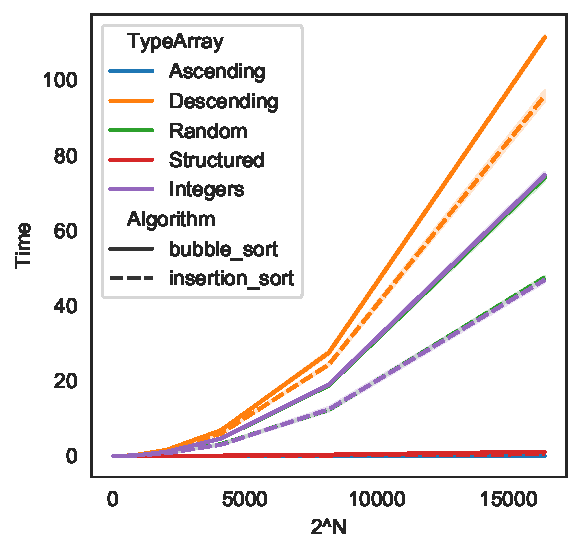
\includegraphics{foo}
  % figure captions below figure
  \caption{Benchmark results for insertion sort and bubble sort.}
  \label{fig:bench}
\end{figure}

Until now have found that insertion sort and bubble sort which are quadratic in time complexity combined with other methods like for example merge sort, drastically reduce sorting time by reducing the callstack and memory complexity. Shown in results, by optimizing the difference beneath merge sort.

\section{Discussion}\label{sec:discussion}

In this section, you should summarize your results and compare them to
expectations from theory presented in Sec.~\ref{sec:theory}.

% In the acks section, you can thank people for help.
\begin{acks}
We are grateful to \dots for \dots.
\end{acks}


%% The next two lines define the bibliography style to be used, and
%% the bibliography file.
\bibliographystyle{ACM-Reference-Format}
\bibliography{References
Iterative Quick Sort - GeeksforGeeks. 2020. GeeksforGeeks. https://www.geeksforgeeks.org/iterative-quick-sort/?fbclid=IwAR2ziWGZKt7nrgiD94kKu2if00gLmh3j2oNR6DUnSsL2b1AoLMsjvpARgYk.}
\bibliography{Insertion sort. 2020. En.wikipedia.org. https://en.wikipedia.org/wiki/Insertion_sort.}
\bibliography{Comparison of Sorting Algorithms. 2020. Medium. https://medium.com/@tssovi/comparison-of-sorting-algorithms-298fdf037c8f.}

\end{document}
